\subsection{Open-loop model of the car}

\begin{figure}
\centering
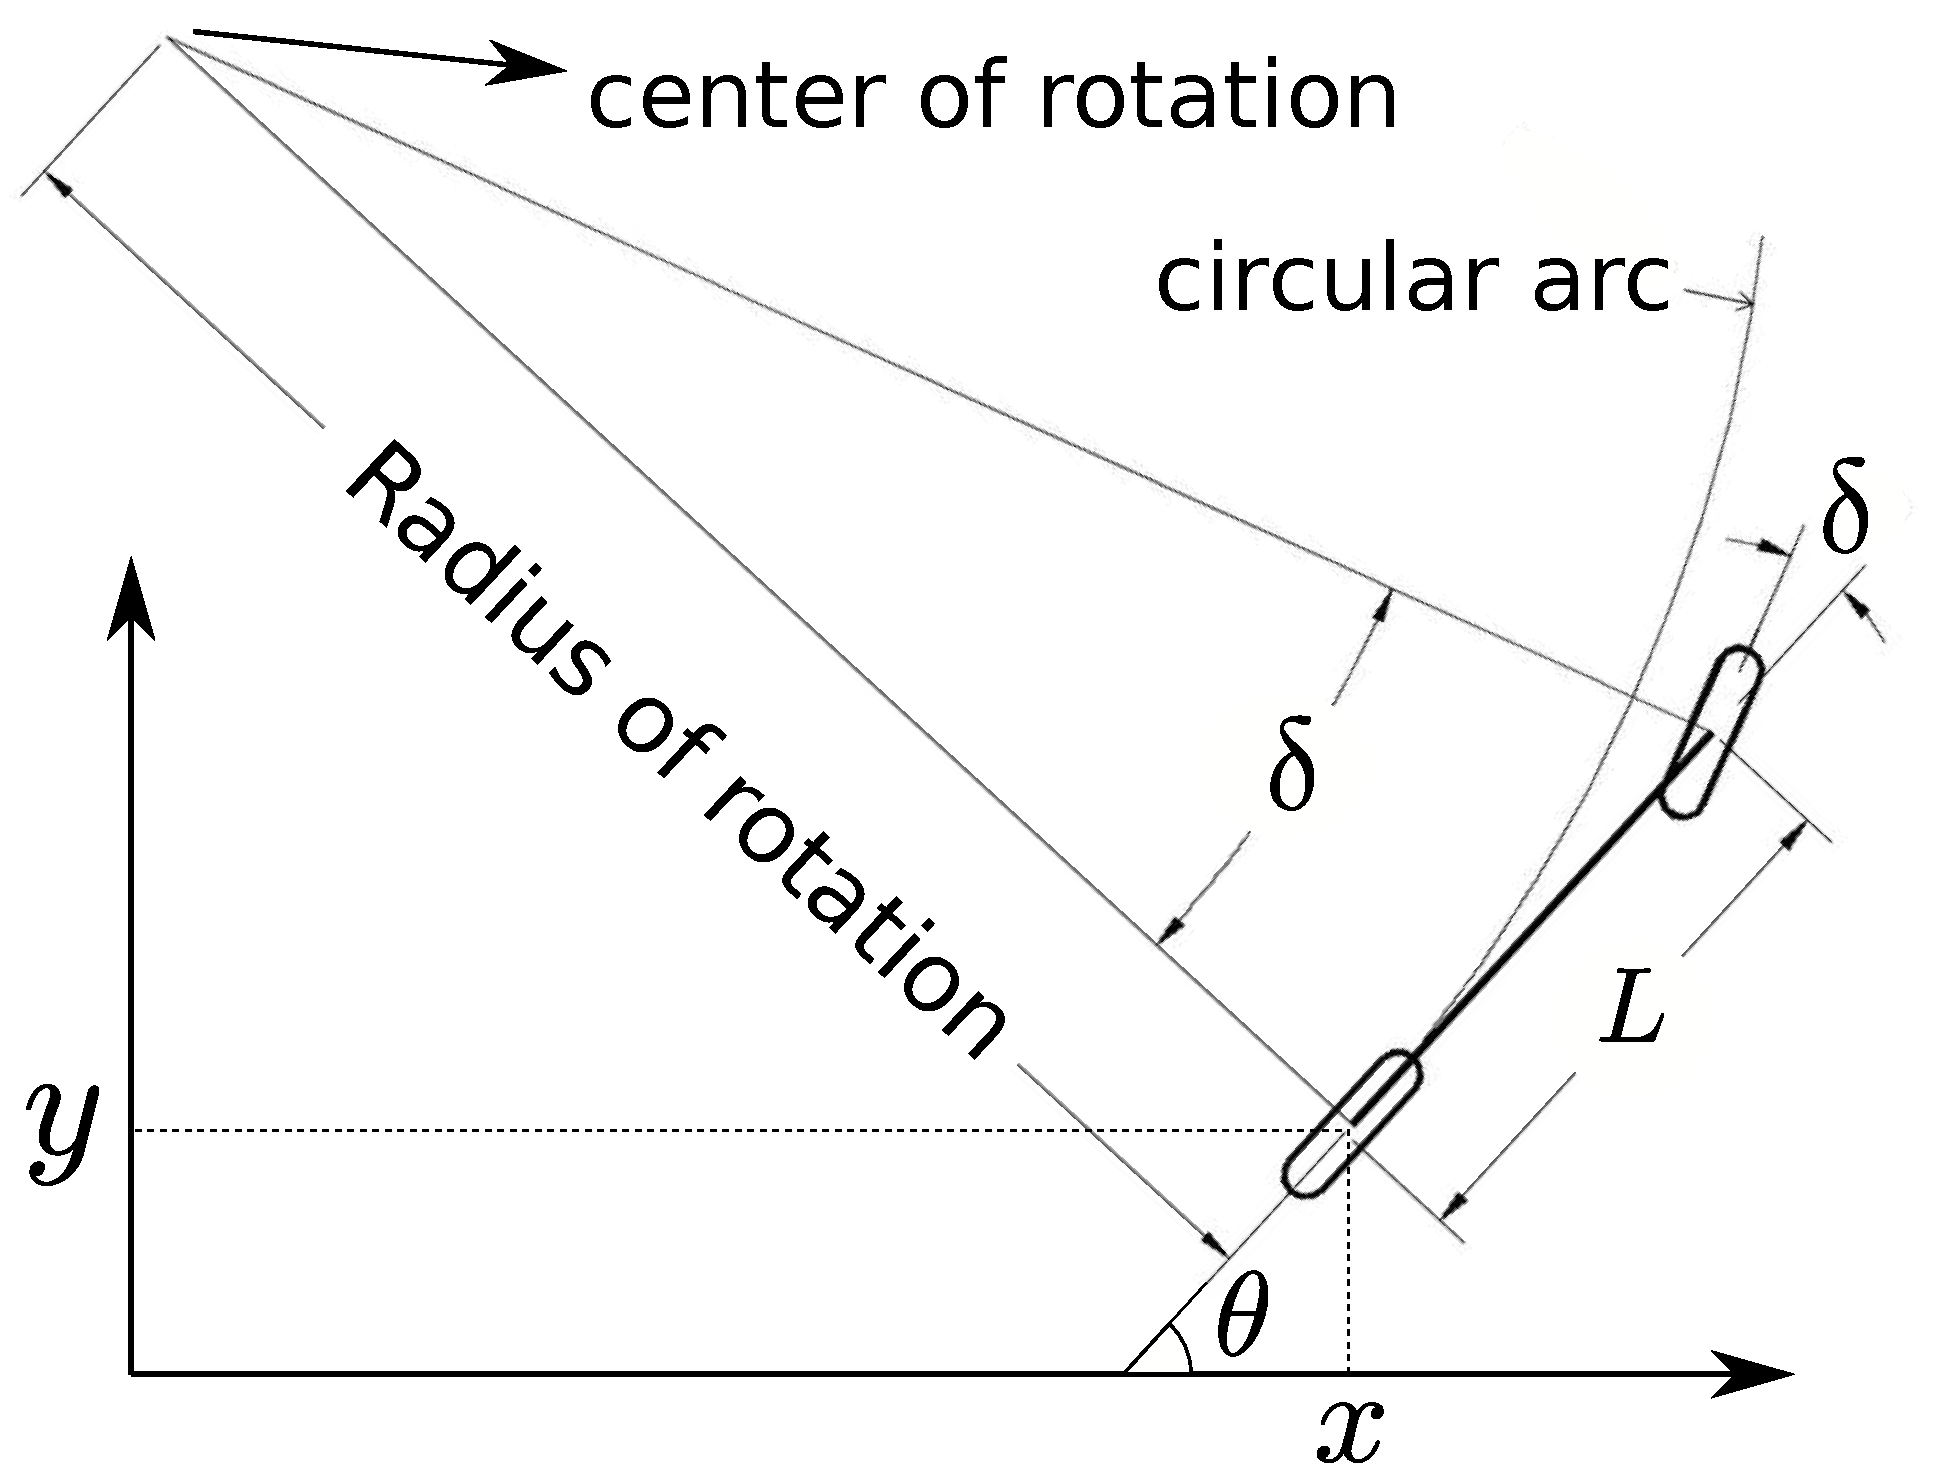
\includegraphics[width=45mm]{Figures/BicycleModel-coords.pdf}%
\caption{Bicycle model \cite{Snider.2009}}
\label{fig:bicycle}%
\end{figure}

The \emph{open-loop} model gives the dynamics of the car as a function of the car's state and input.
%
The \emph{state} is the car's pose (location and orientation) with respect to the map, and the \emph{input} is the steering angle.
%
Here, \emph{open} means that the input can be any function.
%
In contrast, the \emph{closed-loop} model gives the dynamics where the input is a fixed function of the car's state and its environment.


We choose the bicycle model of a car for the open-loop system.
%
The bicycle model has one rear wheel at the center of the rear axle and one front wheel at the center of the front axle.
%
We assume no wheel slippage, and only the front wheel can steer.
%
The \emph{state} of the system at time $t$
is described by the triple $(x(t), y(t), \theta(t))$
where $(x, y)$ are the coordinates of the rear wheel
in some inertial frame, say the racing track, and
$\theta$ is the angle of the heading direction of the bicycle measured from the $x$-axis counter-clockwise.
%
If $v$ is the speed (magnitude of velocity) of the rear wheel,
$L$ is the \emph{wheelbase} (distance between the rear and front wheels),
and $\delta$ is the steering angle,
then
\[
\left\{
\begin{array}{l}
     \dot{x} = v \cdot cos(\theta) \\
     \dot{y} = v \cdot sin(\theta) \\
     \dot{\theta} = \frac{\displaystyle v}{L} tan(\delta)
\end{array}
\right.
\]
%
Illustration of the bicycle model of the vehicle is provided in Figure~\ref{fig:bicycle}.
